\documentclass[tikz,border=6pt]{standalone}
\usepackage{xcolor}
\begin{document}
% Canonical ch-diagram for 11_1^1,-2
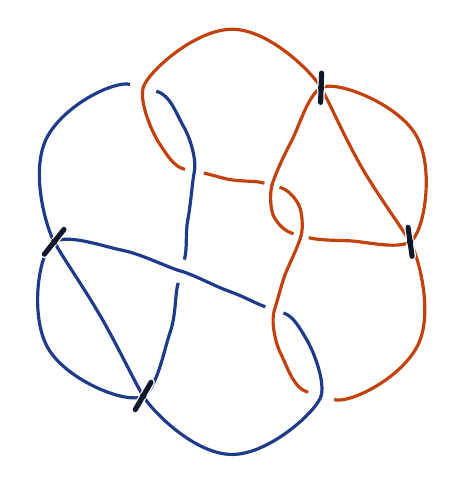
\begin{tikzpicture}[line join=round]
  \definecolor{skcomp0}{RGB}{30,58,138}
  \definecolor{skcomp1}{RGB}{194,65,12}
  \definecolor{skmark}{RGB}{15,23,42}
  \draw[skcomp0, line width=1.15pt, line cap=butt] (-1.2971,2.0001) .. controls (-1.4852,2.0484) and (-2.1002,1.7623) .. (-2.3383,1.3500);
  \draw[skcomp0, line width=1.15pt, line cap=butt] (-0.6856,-0.5206) .. controls (-0.7301,-0.6866) and (-0.7083,-0.9167) .. (-0.7888,-1.1518);
  \draw[skcomp0, line width=1.15pt, line cap=butt] (0.4217,-0.8242) .. controls (0.2917,-0.7802) and (0.1534,-0.6944) .. (-0.0285,-0.6314);
  \draw[skcomp0, line width=1.15pt, line cap=butt] (-0.6065,-0.2254) .. controls (-0.5645,-0.0686) and (-0.5975,0.1020) .. (-0.5611,0.2910);
  \draw[skcomp1, line width=1.15pt, line cap=butt] (-0.5987,0.9209) .. controls (-0.7319,0.9475) and (-0.8246,1.0975) .. (-0.9241,1.2496);
  \draw[skcomp0, line width=1.15pt, line cap=butt] (-0.9628,1.9142) .. controls (-0.7851,1.8686) and (-0.7076,1.6216) .. (-0.6153,1.4625);
  \draw[skcomp1, line width=1.15pt, line cap=butt] (0.9727,0.0529) .. controls (1.0812,0.0242) and (1.2579,0.0203) .. (1.4687,0.0144);
  \draw[skcomp1, line width=1.15pt, line cap=butt] (1.2962,-2.0036) .. controls (1.4833,-2.0558) and (2.1002,-1.7623) .. (2.3383,-1.3500);
  \draw[skcomp0, line width=1.15pt, line cap=butt] (0.6529,-0.9025) .. controls (0.7829,-0.9465) and (0.8673,-1.1046) .. (0.9589,-1.2641);
  \draw[skcomp1, line width=1.15pt, line cap=butt] (0.9637,-1.9107) .. controls (0.7785,-1.8591) and (0.7021,-1.5874) .. (0.6201,-1.4251);
  \draw[skcomp1, line width=1.15pt, line cap=butt] (-0.3594,0.8731) .. controls (-0.2322,0.8477) and (-0.1108,0.7980) .. (0.0346,0.7821);
  \draw[skcomp1, line width=1.15pt, line cap=butt] (0.4097,0.7458) .. controls (0.3017,0.7751) and (0.1800,0.7662) .. (0.0346,0.7821);
  \draw[skcomp1, line width=1.15pt, line cap=butt] (0.7798,0.1039) .. controls (0.6756,0.1314) and (0.5903,0.2150) .. (0.5358,0.3094);
  \draw[skcomp1, line width=1.15pt, line cap=butt] (0.6023,0.6935) .. controls (0.7046,0.6657) and (0.7842,0.5790) .. (0.8389,0.4843);
  \draw[skcomp0, line width=1.15pt, line cap=round] (-2.2599,0.0000) .. controls (-2.1506,-0.1975) and (-1.8750,-0.5922) .. (-1.6626,-0.9599);
  \draw[skcomp0, line width=1.15pt, line cap=round] (-1.1300,-1.9571) .. controls (-1.2463,-1.7637) and (-1.4503,-1.3277) .. (-1.6626,-0.9599);
  \draw[skcomp0, line width=1.15pt, line cap=round] (-2.2599,0.0000) .. controls (-2.0734,0.1033) and (-1.6357,-0.0594) .. (-1.3919,-0.1072);
  \draw[skcomp0, line width=1.15pt, line cap=round] (-0.6461,-0.3730) .. controls (-0.8121,-0.3285) and (-1.1481,-0.1550) .. (-1.3919,-0.1072);
  \draw[skcomp0, line width=1.15pt, line cap=round] (-2.2599,0.0000) .. controls (-2.3693,0.1975) and (-2.5763,0.9377) .. (-2.3383,1.3500);
  \draw[skcomp0, line width=1.15pt, line cap=round] (-2.2599,0.0000) .. controls (-2.4574,-0.1094) and (-2.5763,-0.9377) .. (-2.3383,-1.3500);
  \draw[skcomp0, line width=1.15pt, line cap=round] (-1.1300,-1.9571) .. controls (-1.3234,-2.0735) and (-2.1002,-1.7623) .. (-2.3383,-1.3500);
  \draw[skcomp0, line width=1.15pt, line cap=round] (-1.1300,-1.9571) .. controls (-1.0136,-2.1506) and (-0.4761,-2.7000) .. (0.0000,-2.7000);
  \draw[skcomp0, line width=1.15pt, line cap=round] (1.1300,-1.9571) .. controls (1.0778,-2.1442) and (0.4761,-2.7000) .. (0.0000,-2.7000);
  \draw[skcomp0, line width=1.15pt, line cap=round] (-1.1300,-1.9571) .. controls (-0.9473,-1.8473) and (-0.8693,-1.3869) .. (-0.7888,-1.1518);
  \draw[skcomp0, line width=1.15pt, line cap=round] (-0.6461,-0.3730) .. controls (-0.4893,-0.4150) and (-0.2104,-0.5684) .. (-0.0285,-0.6314);
  \draw[skcomp0, line width=1.15pt, line cap=round] (-0.4790,0.8970) .. controls (-0.5059,0.7624) and (-0.5247,0.4800) .. (-0.5611,0.2910);
  \draw[skcomp1, line width=1.15pt, line cap=round] (-1.1300,1.9571) .. controls (-1.1778,1.7709) and (-1.0237,1.4018) .. (-0.9241,1.2496);
  \draw[skcomp0, line width=1.15pt, line cap=round] (-0.4790,0.8970) .. controls (-0.4521,1.0316) and (-0.5229,1.3034) .. (-0.6153,1.4625);
  \draw[skcomp1, line width=1.15pt, line cap=round] (-1.1300,1.9571) .. controls (-1.0817,2.1452) and (-0.4761,2.7000) .. (0.0000,2.7000);
  \draw[skcomp1, line width=1.15pt, line cap=round] (1.1300,1.9571) .. controls (1.0271,2.1390) and (0.4761,2.7000) .. (0.0000,2.7000);
  \draw[skcomp1, line width=1.15pt, line cap=round] (1.1300,1.9571) .. controls (0.9582,1.8600) and (0.8471,1.4503) .. (0.7468,1.2648);
  \draw[skcomp1, line width=1.15pt, line cap=round] (0.5060,0.7196) .. controls (0.5354,0.8279) and (0.6465,1.0792) .. (0.7468,1.2648);
  \draw[skcomp1, line width=1.15pt, line cap=round] (1.1300,1.9571) .. controls (1.2328,1.7753) and (1.4419,1.2993) .. (1.6440,0.9492);
  \draw[skcomp1, line width=1.15pt, line cap=round] (2.2599,0.0000) .. controls (2.1538,0.1800) and (1.8462,0.5990) .. (1.6440,0.9492);
  \draw[skcomp1, line width=1.15pt, line cap=round] (1.1300,1.9571) .. controls (1.3118,2.0600) and (2.1002,1.7623) .. (2.3383,1.3500);
  \draw[skcomp1, line width=1.15pt, line cap=round] (2.2599,0.0000) .. controls (2.4399,0.1061) and (2.5763,0.9377) .. (2.3383,1.3500);
  \draw[skcomp1, line width=1.15pt, line cap=round] (2.2599,0.0000) .. controls (2.0899,-0.1002) and (1.6796,0.0084) .. (1.4687,0.0144);
  \draw[skcomp1, line width=1.15pt, line cap=round] (2.2599,0.0000) .. controls (2.3660,-0.1800) and (2.5763,-0.9377) .. (2.3383,-1.3500);
  \draw[skcomp0, line width=1.15pt, line cap=round] (1.1300,-1.9571) .. controls (1.1793,-1.7805) and (1.0505,-1.4236) .. (0.9589,-1.2641);
  \draw[skcomp1, line width=1.15pt, line cap=round] (0.5373,-0.8634) .. controls (0.4938,-0.9920) and (0.5382,-1.2628) .. (0.6201,-1.4251);
  \draw[skcomp1, line width=1.15pt, line cap=round] (0.5373,-0.8634) .. controls (0.5789,-0.7406) and (0.6357,-0.4949) .. (0.6946,-0.3611);
  \draw[skcomp1, line width=1.15pt, line cap=round] (0.8762,0.0784) .. controls (0.8476,-0.0299) and (0.7535,-0.2273) .. (0.6946,-0.3611);
  \draw[skcomp1, line width=1.15pt, line cap=round] (0.5060,0.7196) .. controls (0.4778,0.6157) and (0.4813,0.4037) .. (0.5358,0.3094);
  \draw[skcomp1, line width=1.15pt, line cap=round] (0.8762,0.0784) .. controls (0.9033,0.1809) and (0.8935,0.3896) .. (0.8389,0.4843);
  \draw[white, line width=2.8pt, line cap=round] (-2.3845,-0.1572) -- (-2.1353,0.1572);
  \draw[skmark, line width=1.85pt, line cap=round] (-2.3845,-0.1572) -- (-2.1353,0.1572);
  \fill[skmark] (-2.2599,0.0000) circle (1.2pt);
  \draw[white, line width=2.8pt, line cap=round] (-1.0296,-1.7834) -- (-1.2303,-2.1309);
  \draw[skmark, line width=1.85pt, line cap=round] (-1.0296,-1.7834) -- (-1.2303,-2.1309);
  \fill[skmark] (-1.1300,-1.9571) circle (1.2pt);
  \draw[white, line width=2.8pt, line cap=round] (1.1361,2.1428) -- (1.1238,1.7715);
  \draw[skmark, line width=1.85pt, line cap=round] (1.1361,2.1428) -- (1.1238,1.7715);
  \fill[skmark] (1.1300,1.9571) circle (1.2pt);
  \draw[white, line width=2.8pt, line cap=round] (2.2858,-0.1839) -- (2.2341,0.1839);
  \draw[skmark, line width=1.85pt, line cap=round] (2.2858,-0.1839) -- (2.2341,0.1839);
  \fill[skmark] (2.2599,0.0000) circle (1.2pt);
\end{tikzpicture}
\end{document}
